\section{Related work}

\begin{figure*}[ht]
\vspace{-2mm}
\centering
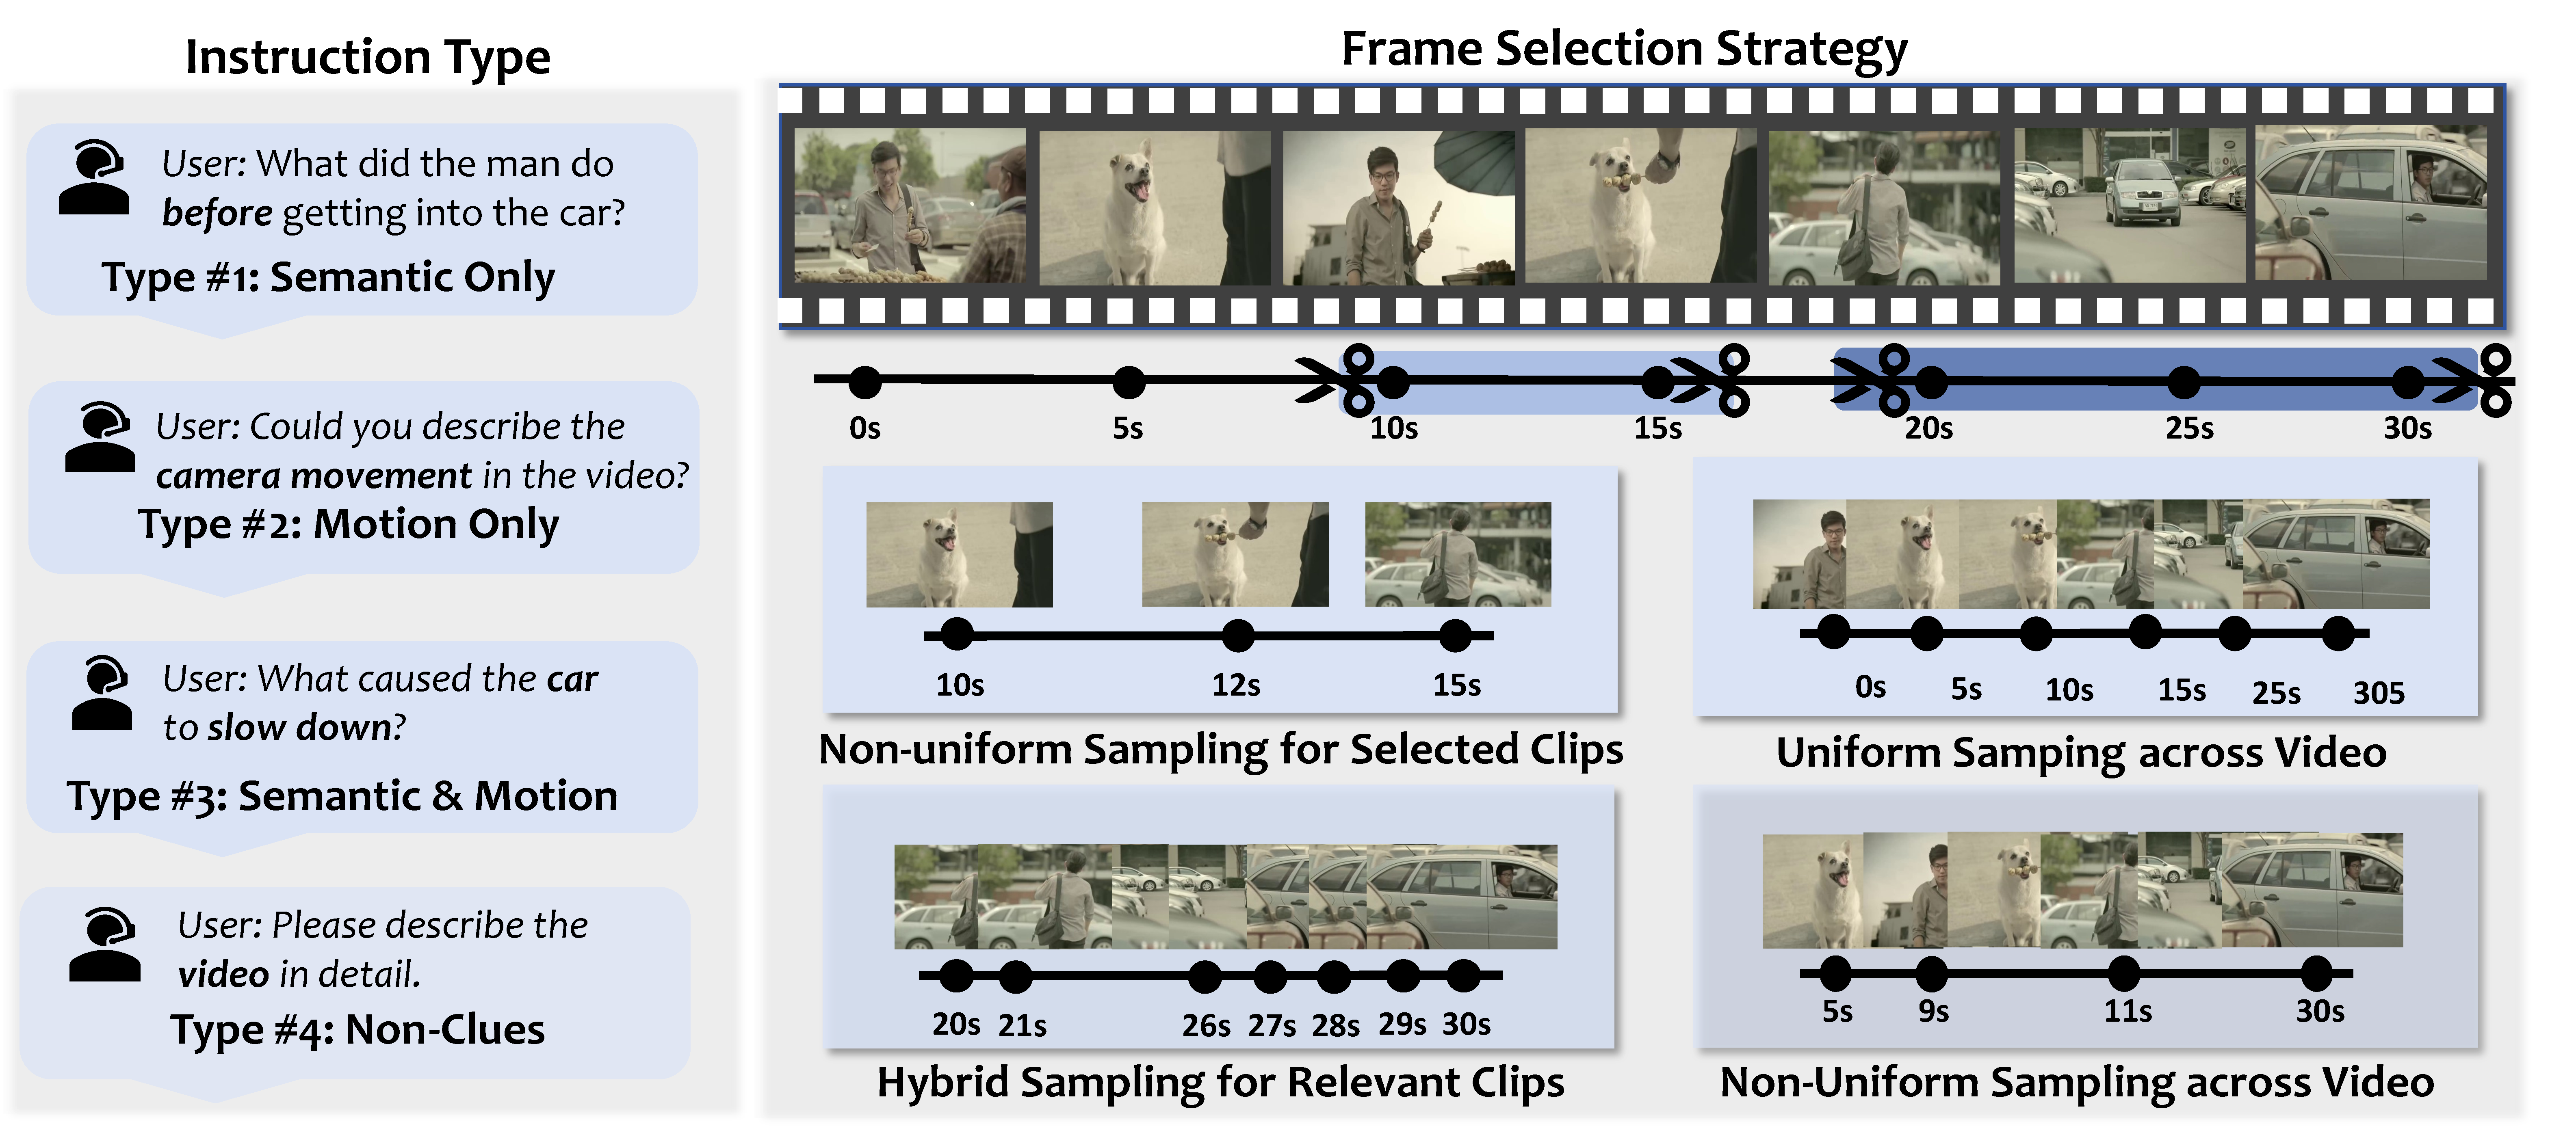
\includegraphics[width=0.96\linewidth]{dataset.pdf}
\vspace{-2mm}
\caption{\textbf{Illustration of four instruction types and their corresponding frame selection strategies in VidThinker.} For semantic-focused instructions, the system selects diverse frames capturing key visual clues. For motion-focused instructions, frames are uniformly sampled to capture dynamic changes. When both semantic and motion cues are required, a hybrid sampling strategy is applied. For vague or open-ended instructions, the system samples a minimal yet diverse set of frames across the video for holistic coverage.}
\label{dataset}
\vspace{-2mm}
\end{figure*}

\noindent \textbf{Video large language models.} Recent advances in Video-LLMs address the temporal and spatial complexity of long videos through several strategies. Visual feature compression~\cite{liu2025oryx, zohar2024apollo, ye2024mplug, wang2024videollamb, liu2025video} is achieved by modules like Q-Former~\cite{song2024moviechat} and Perceiver Resampler~\cite{zohar2024apollo}, which merge frame features into fixed queries. Spatial pooling~\cite{maaz2024video, xu2024slowfast, xu2024pllava} helps preserve long-range temporal information efficiently. Some models extend sequence length for longer inputs~\cite{zhang2024long, wang2024qwen2, team2023gemini, chen2025eagle}, but this often increases computational cost~\cite{wei2024visual, shu2025video}. To reduce redundancy, similarity-based frame filtering is used~\cite{jin2024video, shen2024longvu}, though fixed thresholds may miss real-world diversity. 



\noindent \textbf{Keyframe selection for Video-LLMs.} The goal of keyframe selection is to choose a compact subset of frames that preserves task-critical semantics and temporal evidence while maintaining sufficient video-level coverage for long-form understanding. Recent methods increasingly incorporate user instructions to rank or retrieve frames most relevant to the query and then feed only these keyframes to the downstream Video-LLM~\cite{liu2025boltboostlargevisionlanguage,tang2025adaptive,luo2025quota,yu2025framevoyagerlearningqueryframes,zhang2025q}.
AKS~\cite{tang2025adaptive} performs adaptive sampling guided by temporal characteristics to reduce redundancy without sacrificing content coverage.
Q-Frame~\cite{zhang2025q} introduces a query-adaptive importance estimator with multi-resolution selection, allocating higher resolution to query-critical segments. A subset of methods selects frames via text–video and video-context similarity, scoring alignment under budget constraints~\cite{yu2025framevoyagerlearningqueryframes,yao2025generative}.



% AKS
% QuoTA
% Gen-S
% BOLT
% Frame-VOYAGER
% Q-Frame

\noindent \textbf{Video temporal grounding.}
Video Temporal Grounding~\cite{ren2024timechat, wang2024grounded, qian2024momentor, di2024grounded} is a common task in video understanding that associates specific video moments with their corresponding timestamps, while Temporal Localization focuses on accurately identifying these moments within untrimmed videos~\cite{liu2024bench, anne2017localizing, li2024multi}. Current Video-LLMs~\cite{shen2024longvu, wang2024grounded, huang2024lita} have begun to leverage temporal grounding for frame selection by linking video with temporal cues; however, existing methods~\cite{huang2025frag,yu2023self,yu2025frame} mostly focus on single-time retrieval, which take descriptive annotations as input, limiting their generality and robustness in handling diverse real-world scenarios.

% 总结句：这里要说我们在VideoLLM、Frame Selection、Temporal Grounding三大方向上做了啥

In this paper, our VideoITG leverages instructed temporal grounding, automated annotation, and a plug-and-play design to align sampling with user instructions, achieving superior performance and scalability on multimodal video understanding benchmarks.


